\documentclass[letterpaper,12pt]{article}
\usepackage{tabularx} % extra features for tabular environment
\usepackage{amsmath}  % improve math presentation
\usepackage{graphicx} % takes care of graphic including machinery
\usepackage[margin=1in,letterpaper]{geometry} % decreases margins
\usepackage{wrapfig, blindtext}
\usepackage{graphicx}
\usepackage{placeins}
\usepackage{cite} % takes care of citations
\usepackage[final]{hyperref} % adds hyper links inside the generated pdf file
\hypersetup{
	colorlinks=true,       % false: boxed links; true: colored links
	linkcolor=blue,        % color of internal links
	citecolor=blue,        % color of links to bibliography
	filecolor=magenta,     % color of file links
urlcolor=blue}
%\FloatBarrier


\begin{document}
\title{}
\author{}
\date{}


\begin{center}
\textbf{Traffic Sign Classification - Jack Wetherell} \\
\end{center}


\section{Introduction}
The goals of this project were the following:
\begin{itemize}
\item Load a provided dataset of labelled German traffic signs.
\item Explore, summarise  and visualise the dataset.
\item Design, train and test a deep-learning model architecture in order to classify the traffic signs.
\item Use the model to make predictions on new images, and  analyse the softmax probabilities of the new images.
\end{itemize}
The project notebook contains the source code of this implementation, as well as the results. In addition there are also pdf copies of this notebook available. 
In the next sections I will cover how each of the rubric points have been addressed in this work.

\section{Data Set Summary and Exploration }
I used the python standard library module \texttt{pickle} to load the provided dataset into memory. This was pre-split into a training, validation and test set. I used the \texttt{numpy} library to calculate summary statistics of the traffic signs data set: 
\begin{itemize}
\item Number of training examples = 34799 
\item Number of validation examples = 4410 
\item Number of testing examples = 12630 
\item Image data shape = (32, 32) each with 3 color channels 
\item Number of classes = 43
\end{itemize}
I used \texttt{pandas} to import the csv if class labels and used this to creat a dictionary object to convert between class index (int) and class label (string). Next I visualised 25 random training examples, plotting the image along with the class label in each case (Figure 1a). Next, I plotted the distributions of each class in the train, validation and test sets respectively (Figure 1b) . In order to ensure the train, validation, test split was done correctly, and without any bias, I ensured that the relative count of each of the classes fell on a straight line, to ensure no occurrence bias is present in the splitting (Figure 1c).
\begin{figure}
\centering
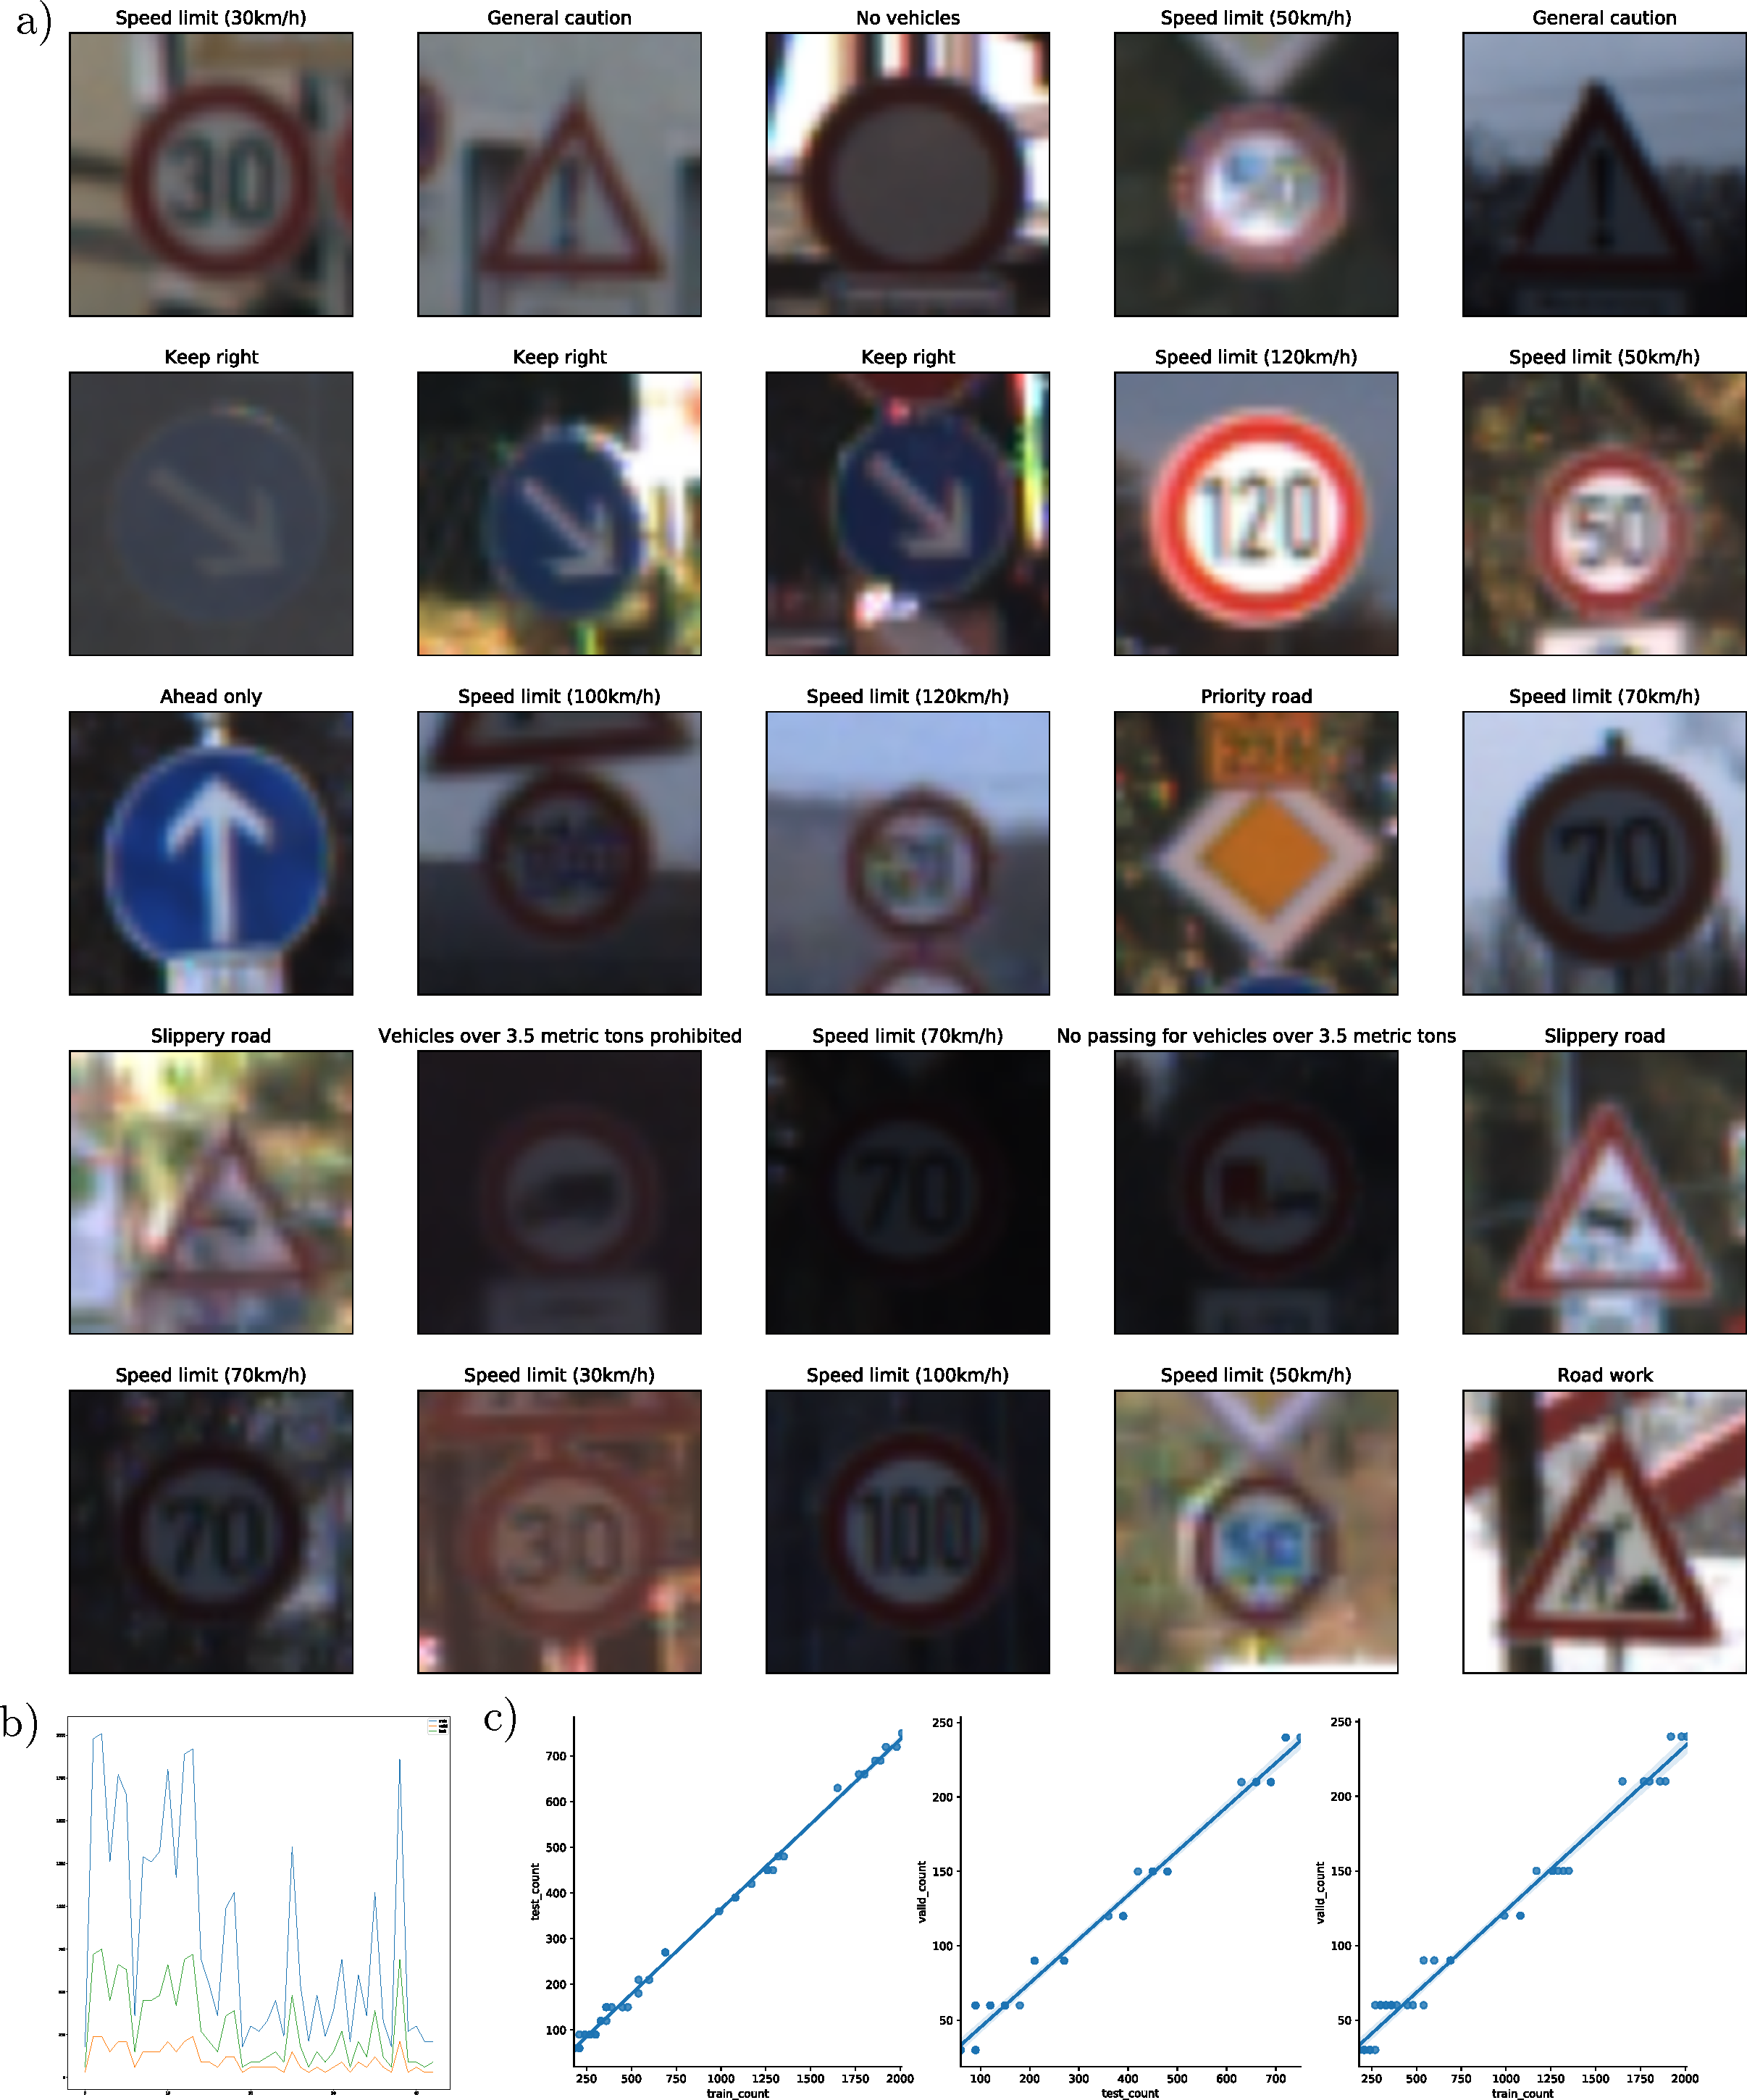
\includegraphics[scale=0.4]{../results/fig1.pdf}
\caption{Data set summary and exploration. Panel a shows 25 random images and respective class labels from the training set. Panel b shows the distributions of the 43 classes within each of the train (blue), validation (yellow) and test (green) sets. Panel 3 shows the plots of the counts of each of the 43 classes for the test, train and validation sets relative to each other, showing they are correctly proportioned.}
\end{figure}
\newpage

\section{Design and Test a Model Architecture}
During my model tuning I used several preprocessing techniques.
\begin{enumerate}
\item I normalised the images such that the values ranged from 0 to 1 rather than the original 0 to 255. This is because this well aligns the inputs with the sale of the randomly initialised normally distributed weights of the CNN.
\item I ensured the data was centred around a mean of zero, insuring that it would result in a statistically well behaved training process. I used \texttt{numpy} to perform this shift of the mean to zero
\item I also shuffled the images, to ensure the order they are presented in training does not result in any systematic bias. This was performed using \texttt{sklearn}. 
\end{enumerate}
I also attempted gray scaling and different color spaces. I used `texttt{opencv} to perform these, but I found no significant improvement the the model performance in the limit of large number of EPOCHS, it only had noticeable effects early in the training. Therefore no color modification took place in the final training.


The final model architecture was a modified LeNet model. The architecture consists of the following layers:
\begin{enumerate}
\item Input: shape = (32, 32, 3)
\item Convolution layer:  output shape = (28, 28, 6), activation = relu
\item Pooling layer: output shape = (14, 14, 6)
\item Convolution layer: output shape = (10, 10, 16), activation = relu
\item Pooling layer: output shape = (5, 5, 16)
\item Flatten layer.  output shape = (400)
\item Fully connected layer: output shape = (150), activation = relu
\item Fully connected layer: output shape = (100), activation = relu
\item Fully connected layer: output shape = (43)
\end{enumerate}
When I first training this modified LeNet model I achieved an accuracy of 91.\%. I noticed that the train performance quickly approached 100\% and so showed clear signs of over fitting, in order to fix this I made several modifications:
\begin{enumerate}
\item Added drop-out with a keep probability of 75\% to each of the fully connected layers.
\item Lowered the learning rate to 0.0009 and increased the number of epochs to 50.
\end{enumerate}
The final hyper-parameters of the model are: \texttt{EPOCHS = 50, BATCH\_SIZE = 150, LEARNING\_RATE = 0.0009, DROP = 0.75}. The final results of the model was:
\begin{itemize}
\item Training Accuracy = 100.0\%
\item Validation Accuracy = 97.0\%
\item Test Accuracy = 95.2\%.
\end{itemize}

\section{Testing the model on new images}
In order to test the model on some new images, I 'drove' around Dresden using Google Street view, and took some screen-shots containing street signs. I used \texttt{opencv} to pre-process the images, extracting the part of the image containing the street sign. I used the perspective transform technique from the lane line finding project. The results of this are shown in the figure 2. As can be seen it correctly categorised all five of the images:
\begin{figure}
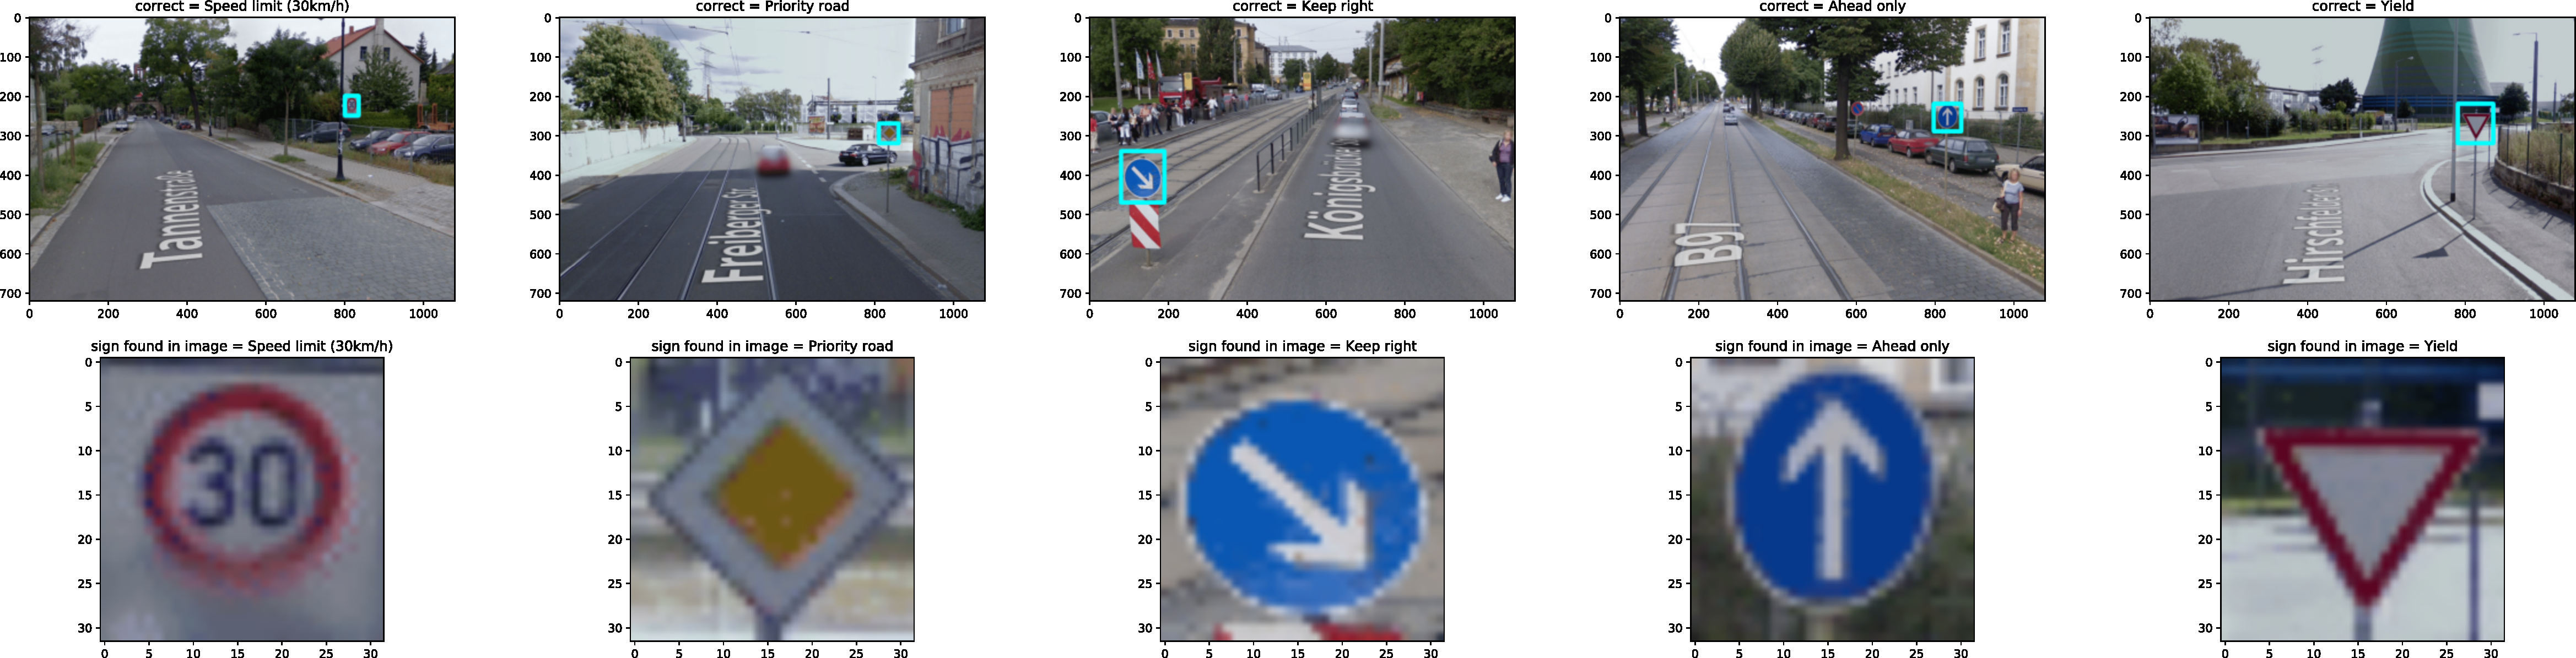
\includegraphics[scale=0.2]{../results/new.pdf}
\caption{Results of applying the model to five signs found 'driving' around Dresden in Google Street View. All five of the signs are correctly classified. }
\end{figure}
The softmax values for each of these cases are 1.0, showing that the model has a high confidence in these predictions. The calculations of these, with the details, is shown in cell 13 of the project notebook.
\end{document}